%******************************************************************************************************
%******************************* Fourth Chapter *******************************************************
%******************************************************************************************************

\externaldocument{{../Chapter1/chapter1}}
\externaldocument{{../Chapter2/chapter2}}
\externaldocument{{../Chapter3/chapter3}}
\externaldocument{{../Chapter5/chapter5}}

% **************************** Define Graphics Path **************************
\graphicspath{{Chapter4/Figs/}}


%******************************************************************************************************
%******************************************************************************************************
\chapter{Task Two: Path Following}
\label{task2}

This is the second of two tasks carried out in this project. Whilst our previous task was aimed at planning paths on the ground prior to flight, this task is aimed at commanding the UAV to fly such paths.


%******************************************************************************************************
%******************************************************************************************************
\section{Path Following - Aims}
\label{task2:aims}

The overarching aim for this task is to implement changes to ArduPlane to allow us to fly an air relative Dubins path as defined by the work already completed. Thanks to our path planning solution the UAV does not need to be aware of its ground relative location in order to successfully navigate to our desired point. The path following solution must simply interpret our description of a Dubins path and perform the desired manoeuvres. 

We need to be able to take a mission plan created using MissionPlanner or APM Planner 2 and insert a series of flight commands that will result in the UAV flying our desired Dubins path. To do this, we need to define the these commands in a format the autopulot will understand, and then enable the autopilot to respond to these input commands. 

We can summarise this tasks as being aimed at achieving the following:

\begin{itemize}
	\item Being able to describe a Dubins path using MAVLink messages %TODO introduce mavlink messages
	\item Enabling the UAV to interpret and act upon the new MAVLink messages
	\item Successfully command the UAV to fly a Dubins path, both with and without the presence of wind
	\item Successfully commanding the UAV to fly in wind to a ground relative point using a Dubins path 
\end{itemize}

From these aims, we can define a number of stages to split this task into, as we did with the previous task. Doing so simplifies design, implementation, and testing, whilst also providing clear milestones and cut off points to work well with the planning processes used in this project.These stages were defined as:

\begin{enumerate}
	\item Define the format of new commands required to fly a Dubins path
	\item Enable the UAV to interpret newly added commands
	\item Command the UAV to fly a Dubins path in both the presence and absence of wind
\end{enumerate}

Stage 1 comprises of design, implementation and testing. Stage 2 is purely design and implementation, whilst Stage 3 is a primarily testing phase.  

%******************************************************************************************************
%******************************************************************************************************
\section{Path Following - Stage 1: Defining New Flight Commands}
\label{task2:stage1}

In this section we shall follow the design, implementation, and testing phases completed in order to define our new flight commands. This work prepares us for the next stage of adding functionality to ArduPlane so as to read, interpret, and act upon the new commands we have provided. 

\subsection{Stage 1: Design and Implementation}
\label{task2:stage1:design}

ArduPilot products use MAVLink messages to define all of the commands that may be included in a mission plan; a full list of the current MAVLink messages can be seen at \cite{MavlinkMessages}. A complete mission plan will simply be a collection of MAVLink messages, where each line corresponds to one MAVLink message, consisting of the following fields:

\begin{itemize}
	\item INDEX - an identifier for each command
	\item CURRENT WP - indicating which waypoint the command relates to (irrelevant for this project)
	\item COORD FRAME - indicates whether altitude values are relative to the takeoff altitude or to previous waypoint altitude
	\item COMMAND - the command number used to identify each instruction in the mission plan
	\item PARAM1 - optional parameter field
	\item PARAM2 - optional parameter field
	\item PARAM3 - optional parameter field
	\item PARAM4 - optional parameter field
	\item PARAM5/X/LONGITUDE - optional parameter field or a GPS longitude value 
	\item PARAM6/Y/LATITUDE - optional parameter field or a GPS latitude value
	\item PARAM7/Z/ALTITUDE - optional parameter field or an altitude value
	\item AUTOCONTINUE - flag to indicate whether to continue through the mission plan after this command
\end{itemize}

 To keep our system as simple as possible, it was decided that the easiest way to describe a Dubins path using MAVLink messages was to generate an individual message for each segment of the path. This would allow us to create a MAVLink message that indicated whether the segment needed to be a left-hand turn, right-hand turn, or a straight line. The console application created for path planning accepts the UAV's airspeed as an inpurt argument, and outputs the path as three segments and displays their length. This meant that it was very simple to create a MAVLink message indicating just two things; the segment turn direction, and the duration for the UAV to fly it. 

 As our paths had been designed independent of GPS co-ordinates, each MAVLink message only needed to include the command value, and the duration value in one of the parameter fields. We didn't need any GPS or altitude information in PARAM5, PARAM6, or PARAM7. By following the information found in the developer's wiki at \cite{ArduPilotMAVLink}, we were able to add four new commands. As we knew that our new commands were to be navigation commands, we followed the MAVLink convention of starting the names with ``MAV\_CMD\_NAV\_''. We decided to name our new messages as follows:

 \begin{enumerate}
 	\item MAV\_CMD\_NAV\_DUBIN\_LEFT
 	\item MAV\_CMD\_NAV\_DUBIN\_RIGHT
 	\item MAV\_CMD\_NAV\_DUBIN\_STRAIGHT
 	\item MAV\_CMD\_NAV\_DUMMY\_WP
 \end{enumerate}

 The last command was a dummy command, included so that we would be able to include one of these commands into a simulation, print out a message into the simulator console and therefore be confident that our commands were being read correctly by the autopilot. As the name would suggest, this final command was never intended to do anything other than provide a verification technique.

 The new message types were defined in \path{.../ardupilot/libraries/GCS_MAVLINK/message_definitions/ardupilotmega.xml}. This is the file where developers add platform specific commands, not intended to be shared with other ArduPilot products such as ArduCopter; this is because GCS\_MAVLINK is a shared library, in which most MAVLink messages are defined in the file \path{.../ardupilot/libraries/GCS_MAVLINK/message_definitions/common.xml}.

 An example of one of these definitions is as follows:

 \begin{minipage}{\linewidth}
\begin{lstlisting}[language=XML]
<entry name="MAV_CMD_NAV_DUBIN_RIGHT" value="86">
	<description>Perform a RIGHT turn segment of a dubins path turn</description>
	<param index="1">Duration of time to fly this segment</param>
	<param index="2">Empty</param>
	<param index="3">Empty</param>
	<param index="4">Empty</param>
	<param index="5">Empty</param>
	<param index="6">Empty</param>
	<param index="7">Empty</param>
</entry>
\end{lstlisting}
\end{minipage}

The numerical value chosen for each command is very important, as we have to ensure that all MAV\_CMD\_NAV entries are below 95, which is the value of the MAV\_CMD\_NAV\_LAST command, whilst also ensuring we are using values not currently in use. After double checking their values, the value 84 was assigned to the dummy command, 85 to the left hand turn command, 86 to a right hand turn command, and 87 to a straight segment. By running the \textit{generate.sh} script in the GCS\_MAVLINK directory we finalised this stage of the task, inserting our new commands into the header files used by ArduPlane to interpret MAVLink messages.

\subsection{Stage 1: Testing}
\label{task2:stage1:testing}

The changes produced by this stage were hard to truly test, however would be tested very thoroughly in later stages. The only real testing that was able to be performed at this stage was a visual inspection of the new header files produced. Browsing to \path{...ardupilot/libraries/GCS_MAVLink/include/mavlink/v1.0/ardupilotmega/ardupilotmega.h} confirmed that all four of our new commands were present in the MAV\_CMD enum structure, along with the descriptions and correct command numbers entered in the XML file discussed above. 

%******************************************************************************************************
%******************************************************************************************************
\section{Path Following - Stage 2: Utilising New Flight Commands}
\label{task2:stage1}

In this section we discuss the designand implementation process of enabling ArduPlane to read and interpret our newly defined mission commands. The implementation discussed here is the final and current version created as part of this project, however it was by no means the first method attempted. Further information regarding different approaches to solving this problem will be discussed in Chapter %TODO reference planning problems etc

\subsection{Stage 2: Design and Implementation}
\label{task2:stage2:design}

The design of our final implementation is in fact very simple. The first step towards completing this stage is to convert the MAVLink message into a \textit{cmd} structure, as described in \cite{ArduPilotMAVLink}. To do this we add a case for each of our new commands to the function \textit{mavlink\_to\_mission\_cmd} in \path{...ardupilot/libraries/AP_Mission/AP_Mission.cpp}. Each command issued to the autopilot via a MAVLink message is converted into an instance of a \textit{cmd} structure, which is itself composed of variables as well as a number of other data structures. To convert our message into one of these structures, we fill a data field in a \textit{Dubins\_Duration\_Command} structure, simply used to store the duration value for how long we wish to travel that given segment. This \textit{cmd} structure is then stored in memory, and will be accessed when it is time to complete the associated command. 

The next step is to instruct the autopilot to perform an action upon executing each of these commands. At the heart of ArduPlane is its scheduler, which it uses to periodically call a number of functions which include GPS updates, logging updates, and importantly, navigation updates. Fig. \ref{fig:navigateFlow} shows the program flow that occurs when the scheduler calls the \textit{navigate} function. This is only a small section of the state machine that runs ArduPlane, as a full diagram would be incredibly large and superfluous for this report. 

As can be seen towards the bottom of the flow diagram, there is a point at which we call the \textit{AP\_Mission::update()} function, which asseses whether or not we are currently executing a mission command. In \textit{Plane.h} we initialise an instance of an \textit{AP\_Mission} class with callback pointers to \textit{Plane::start\_command\_callback} and \textit{Plane::verify\_command\_callback}. These functions are both found in \path{...ardupilot/ArduPlane/commands_logic.cpp}, and are responsible for starting each of our mission commands, and verifying that they are complete. This design, whilst a little hard to follow, allows the ArduPilot products to share a huge number of generic libraries, including the \textit{AP\_Mission} library.  


\begin{figure}[htbp!] 
\centering    
\includegraphics[height=0.9\textheight]{Navigate_FlowDiagram}
\caption[ArduPlane's update navigation program flow]{Flow diagram depicting how ArduPlane updates its navigation system}
\label{fig:navigateFlow}
\end{figure}

Within the \textit{commands\_logic.cpp}, the \textit{start\_command\_callback()} function calls the \textit{start\_command} function. We have extended this to include our new functions, as seen in Fig. \ref{fig:startcommand}. Similar additions have been made to the \textit{verify\_command()} function. 

\begin{figure}[htbp!] 
\centering    
\includegraphics[height=0.5\textheight]{StartCommand_FlowDiagram}
\caption[Switch case to select the necessary command to execute]{A simple display of how the Dubins turn commands are called}
\label{fig:startcommand}
\end{figure}

As seen in Fig. \ref{fig:navigateFlow}, the system works by first starting each command, which in turn calls a \textit{do\_} function in \textit{commands\_logic.cpp}; for example when starting our dummy command, the function \textit{do\_dummy\_command()} is called. Following this, and once a command has been started, the system will repeatedly call the corresponding \textit{verify\_} command until it returns true. 

Our first step during implementation was to include our dummy functions. The \textit{do\_dummy\_command()} sends a message to the connected ground station, and the \textit{verify\_dummy\_command()} simply returns a true value the first time it is called. When used within the flight simulator, messages sent to a ground control station in fact appear in the simulator console window, offering a technique for us to degub and verify commands during flight, as well as being able to view the flight logs after. This command helped to verify that these new commands were being read correctly and handled by the task scheduling system. 

Following this the \textit{do\_} and \textit{verify\_} commands were added for each of our turn segment commands. The \textit{do\_} commands utilise a \textit{dubin\_segment} structure defined in \textit{Plane.h} which has the following fields:

\begin{minipage}{\linewidth}
\begin{lstlisting}[language=C++]
// Struct for dubins turns storage
struct {
    uint32_t duration_ms; // time to be turning left, for example, in milliseconds
    uint32_t start_time_ms; //Time at which the command started, in milliseconds
    uint32_t end_time_ms; //Time at which the command should end, in milliseconds
}dubin_segment;
\end{lstlisting}
\end{minipage}

We populate the \textit{duration\_ms} field from the parameter stored in the \textit{cmd} structure, and the \textit{start\_time\_ms} by calling a function to return the system time, in milliseconds. The \textit{end\_time\_ms} field is filled by summing the two other values; this field was not strictly necessary, however was left in after being included for some debugging as it makes the code even easier to understand. 

The \textit{verify\_} commands are also all similar, operating using the following code:

\begin{minipage}{\linewidth}
\begin{lstlisting}[language=C++]
bool Plane::verify_dubin_left(const AP_Mission::Mission_Command &cmd)
{

    // If this is the first run, set the start time in millis
    if (dubin_segment.start_time_ms == 0) {
        gcs_send_text_fmt(PSTR("Starting dubin_left with duration %d"), dubin_segment.duration_ms);
        // Set the start time and end time. Don't really need both, but using for debugging
        dubin_segment.start_time_ms = millis();
        dubin_segment.end_time_ms = dubin_segment.start_time_ms + cmd.content.dubins.duration_ms;
    }
    // If the system time is past the end time for the command, return true
    if (dubin_segment.end_time_ms <= millis()) {
        return true;
    } else {
        return false;
    }
} 
\end{lstlisting}
\end{minipage}

Once these were in place, the system needed to be extended to command the UAV to roll in accordance with the Dubins segment it was to be performing. Fig. \ref{fig:updateFlow} shows the program flow that occurs when the scheduler calls the \textit{update\_flight\_mode()} function.

\begin{figure}[htbp!] 
\centering    
\includegraphics[height=0.5\textheight]{Update_FlowDiagram}
\caption[Scheduled program flow to update the current ArduPlane flight mode]{The program flow when the scheduled \textit{update\_flight\_mode()} function is called}
\label{fig:updateFlow}
\end{figure}

Within the \textit{handle\_auto\_mode()} function, a series of commands to dictate the roll, speed, and pitch of the aircraft were included. The following code snippet is taken from this very function; there are other case conditions for other flight commands later on in the code:

\begin{minipage}{\linewidth}
\begin{lstlisting}[language=C++]
switch(nav_cmd_id) {
    case MAV_CMD_NAV_DUBIN_LEFT:
        nav_roll_cd = -(roll_limit_cd/1);
        calc_nav_pitch();
        calc_throttle();
        break;
    case MAV_CMD_NAV_DUBIN_RIGHT:
        nav_roll_cd = (roll_limit_cd/1);
        calc_nav_pitch();
        calc_throttle();
        break;
    case MAV_CMD_NAV_DUBIN_STRAIGHT:
        nav_roll_cd = 0;
        nav_pitch_cd = 0;
        break;
\end{lstlisting}
\end{minipage}

The \textit{nav\_roll\_cd} variable is used to set our roll angle, measured in centi-degrees (100ths of a degree), and \textit{roll\_limit\_cd} is the upper limit for the roll angle (again in centi-degrees) at which our UAV is permitted to fly. The \textit{roll\_limit\_cd} value is dictated by a parameter specific to the UAV platform in use. The default aircraft used by the flight simulator specifies its maximum roll angle as being 65 degrees, or 6500 centi-degrees. 

%TODO maybe small testing section here? dunno

%******************************************************************************************************
%******************************************************************************************************
\section{Path Following - Stage 3: Flying Dubins Paths}
\label{task2:stage3}

This stage of the task was aimed at testing the performance of our work as a whole, incorporating both our path planning application from Chapter 3 and our newly extended ArduPlane code. 

The first test carried out, part way through the implementation stage, was to check that the dummy command implemented printed out a message as expected when included in a mission plan. This was very quick to confirm, and the desired message appeared in the console shortly followed by a message indicating the next mission command was being executed. This proved that the newly defined MAVLink messages were being read properly, and that the \textit{do\_} and \textit{verify\_} commands were working as intended.

\subsection{Dubins Paths in the Absence of Wind}
\label{task2:nowind}

As mentioned in Chapter 3, it was known from early on in the project that this solution would not be perfect. A flight plan formed using a Dubins path would require the UAV to instantaneously roll from it maximum positive roll angle, to its maximum negative roll angle when switching from a right hand turn segment to a left hand turn segment. Accordingly, the next phase of this testing was to determine just how big a problem this would prove to be, and if there was a way to mitigate it with our current path following implementation. 

Using the simulator, we know the roll angle at which we will be commanding our UAV to turn using. We can also specify the airspeed at which to fly, using a \textit{MAV\_CMD\_DO\_CHANGE\_SPEED} command included in the mission plan. This is important, as otherwise the airspeed of the UAV changes regularly during navigation, resulting in inconsistent turning radii. Using these parameters, we are able to calculate our turning radius.


In order to calculate the turning radius of the UAV, a short derivation needs to be explained first. Fig. \ref{fig:bankedTurns} shows the three main forces at play when performing a banked turn; gravity, lift generated by the aircraft, and centipetal force. %TODO reference wikipedia page

\begin{figure}[htbp!] 
\centering    
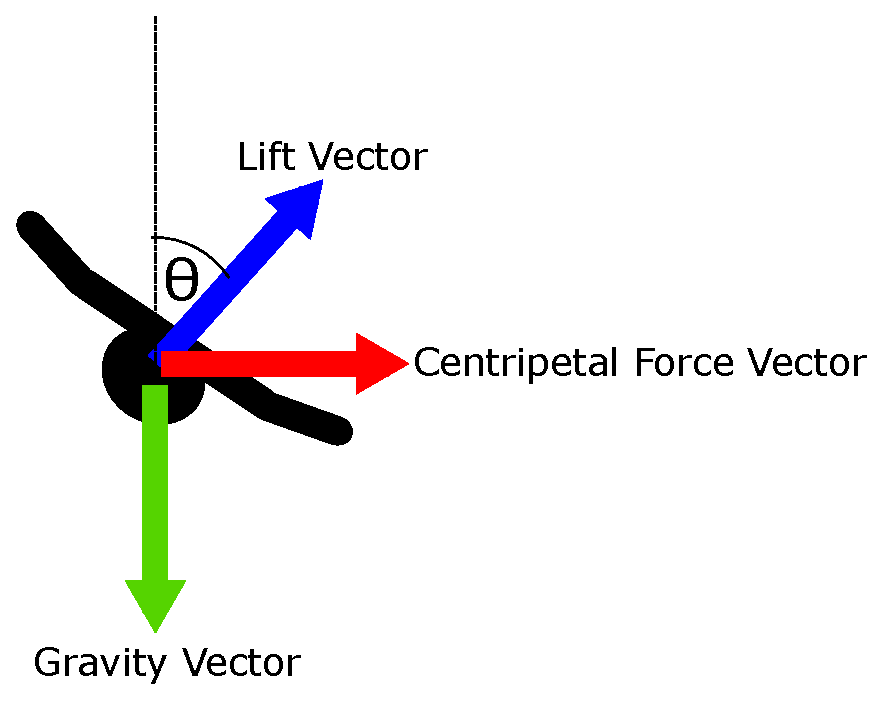
\includegraphics[height=0.4\textheight]{BankedTurns}
\caption[The forces involved in banked turns]{A display of the force vectors affecting the turning radius of an aircraft through a banked turn}%TODO captions
\label{fig:bankedTurns}
\end{figure}

The centripetal force will generate acceleration, defined as:

\begin{equation}
	a = \frac{v^2}{r}	
\end{equation}

where $v$ is the airspeed of the UAV, and $r$ is the turning radius. Newton's second law of motion states that force equals mass times acceleration, and reads:

\begin{equation}
	F = ma
\end{equation}

where $F$ is force, $m$ is mass, and $a$ is acceleration. Substituting this into the equation for centripetal acceleration gives us:

\begin{equation}
	F = \frac{mv^2}{r}	
\end{equation}

 If we define the lift as $L$, we can say that the centripetal force is:

\begin{equation}
	Lsin(\theta)
\end{equation}

where $\theta$ is our bank angle. Therefore:

\begin{equation}
	Lsin(\theta) = \frac{mv^2}{r}
\end{equation}

When in straight and level flight, the lift force must equal the weight of the aircraft, so we can say:

\begin{equation}
	L = mg
\end{equation}

where $g$ is the force of gravity and $m$ is the mass of the aircraft. When turning, the lift increases to become:

\begin{equation}
	L = \frac{mg}{cos\theta}
\end{equation}

Substituting this into our equation for centripetal force:

\begin{equation}
	\frac{sin(\theta)mg}{cos\theta} = \frac{mv^2}{r}
\end{equation}
 
 becomes:

\begin{equation}
	gtan(\theta) = \frac{v^2}{r}
\end{equation}

therefore:

\begin{equation} \label{eq:turnradius}
	r = \frac{v^2}{gtan(\theta)}
\end{equation}

Now that the turning radius and the airspeed are known quantities, a mission plan can be generated. The process for creating a mission plan to perform a Dubins path turn is as follows:
\begin{enumerate}
	\item Create a regular mission plan using waypoints in either MissionPlanner or APM Planner 2, making note of which path sections should be treated as imaging paths
	\item Measure distances between end points of imaging paths
	\item Calculate desired UAV orientation at each point
	\item Use console application to find the suitable Dubins path in the form of three segment lengths and turn directions
	\item Insert new commands into mission plan between the relevent waypoints
\end{enumerate}

An example of one of these mission plans can be seen in Appendix %TODO appendix a mission plan

A mission plan was created to fly the mission displayed in Appendix %TODO appendix screenshot of mission planner
, performing Dubins path turns at waypoint 2, between waypoints 3 and 4, 5 and 6, and at waypoint 7. When performing one of these new turns about a single waypoint, the technique is being used in attempt to only re-align the UAV with the path, as opposed to translating the position of the UAV as well as re-aligning it. 

In the first test of the finished system, the UAV was commanded to fly at 20 metres per second airspeed, in the absence of wind. Fig. \ref{fig:6520nowind} shows both the planned route, and the route the UAV actually flew. Please note that the waypoint numbering in the simulator becomes inaccurate once the additional commands are added to the mission plan. 

As we can see, the UAV is failing to correctly align itself with our imaging paths, with respect to both location and orientation. Inspection of the figure shows that for turns requiring a greater overall turn angle, the errors are far more prevalent than turns requiring a smaller overall turn angle. In particular, the first of the new turning commands resulted in an orientation error of around 90 \degree. Later testing showed that the errors on the first corner were massively exacerbated by speed; although commanding the UAV to fly at a certain airspeed, for some unknown reason it was not doing so. Instead it was flying at greater speeds, thus increasing our turning radius.

\begin{figure}[htbp!] 
\centering    
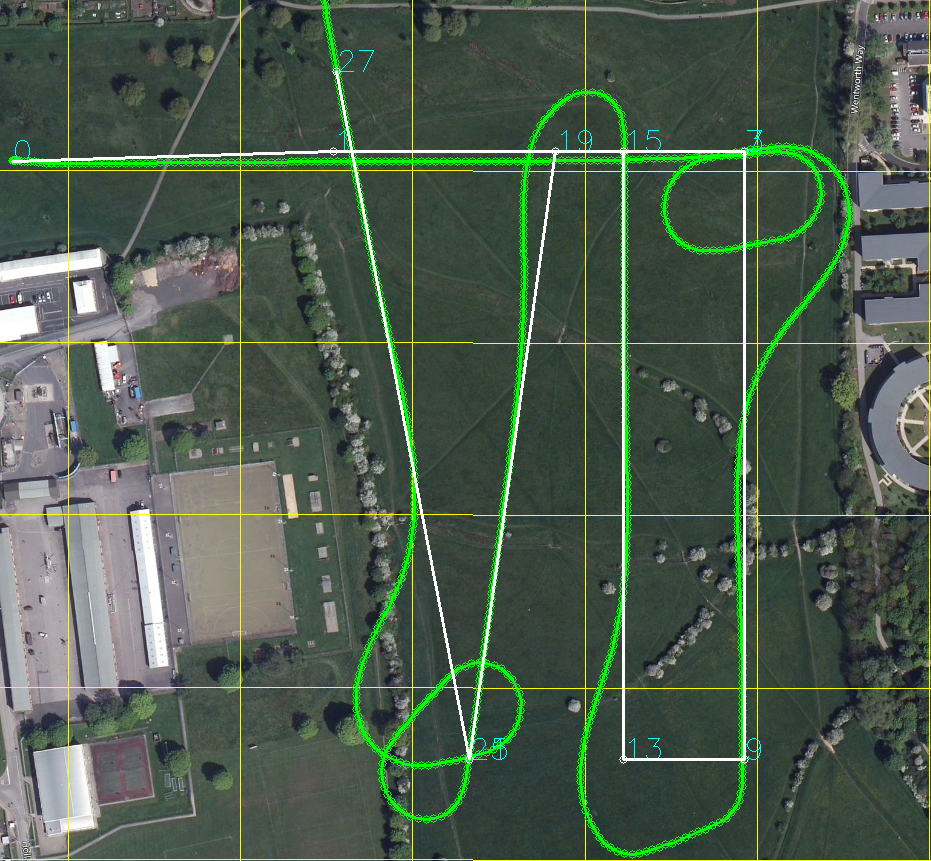
\includegraphics[width=\textwidth]{65_20_NoWind}
\caption[Flying Dubins path turns in the absence of wind]{}
\label{fig:6520nowind}
\end{figure} 

As early as the planning stage, it was known that the time taken to roll the aircraft to the desired angle would have a negative impact on the path following ability of this system. This first test showed just how severe it was, and prompted further investigation into this error. In order to determine how a number of factors impacted this, a special mission was created. This mission commanded the UAV to take off and adjust its speed, then fly the following Dubins path segments:

\begin{enumerate}
	\item Straight segment for 4 seconds
	\item Left turn segment for 4 seconds
	\item Right turn segment for 4 seconds
	\item Straight segment for 4 seconds
	\item Right turn segment for 4 seconds
	\item Left turn segment for 4 seconds
	\item Straight segment for 4 seconds
\end{enumerate}

This series of commands creates 6 transitionas between Dubins path segments. Performing them in this order shows all possible transitions variations, in the fewest number of turns. They can be displayed as:

\begin{enumerate}
	\item S \textrightarrow L
	\item L \textrightarrow R
	\item R \textrightarrow S
	\item S \textrightarrow R
	\item R \textrightarrow L
	\item L \textrightarrow S
\end{enumerate}

This mission plan, availabe in Appendix %TODO appendix roll test mission plan
, was then flown with the same configuration as for the test shown in Fig. \ref{fig:6520nowind}; namely, with a maximum roll angle of 65\degree and at an airspeed of 20 metres per second. 

By opening the \textit{.BIN} log file in MissionPlanner, it is possible to convert it into a MATLAB \textit{.mat} file. Processing the results in MATLAB, the values for commanded roll and actual roll were plotted, as seen in \ref{fig:6520cursors}. 

\begin{figure}[htbp!] 
\centering    
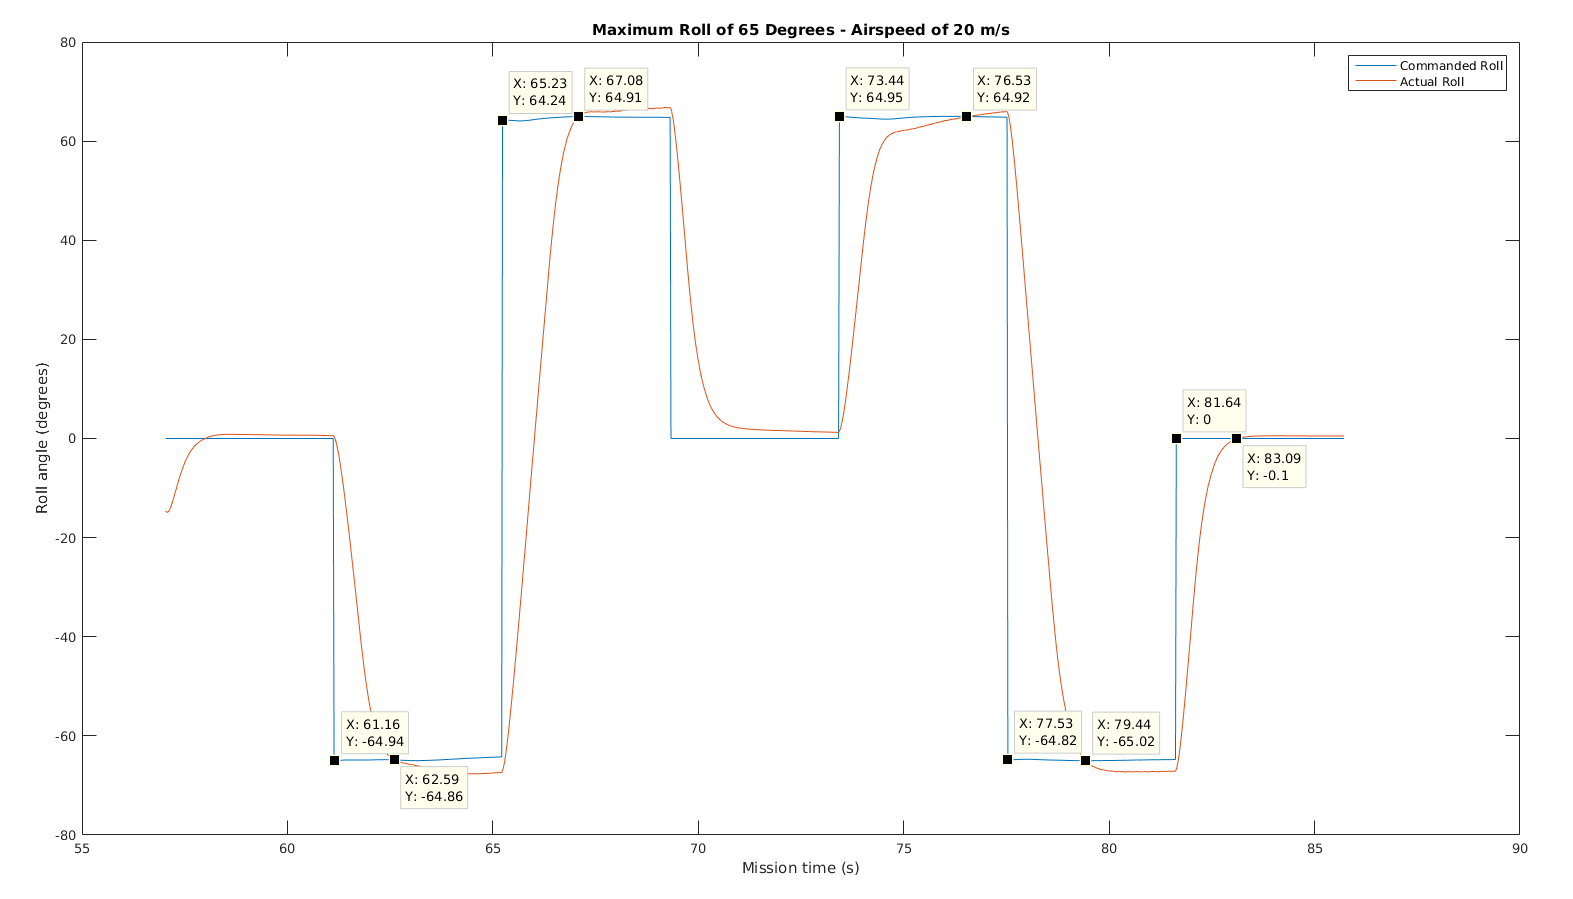
\includegraphics[angle=90,height=0.9\textheight]{65_20_cursors}
\caption[Comparing commanded roll angle with actual roll over time]{A comparison of the commanded roll angle with the actual roll angle over time, displaying the time delay between an angle being commanded and being achieved}
\label{fig:6520cursors}
\end{figure} 

These results clearly show that there is considerable lag between the roll command being issued, and the roll angle being reached. Additional to this problem is the actual roll behaviour being inconsistent; in some scenarios it overshoots its desired roll angle, and in others it does not reach it at all. The two types of roll scenario being displayed here are a change in the roll angle equivalent to the maximum roll angle (0\degree to +/-65\degree, or vice versa), and a change equivalent to double the maximum roll angle (+/-65\degree to-/+65\degree). Interestingly, there seems to be very little difference in time delay between these two scenarios, with both roughly equalling a 2 second lag. Continuing this investigation, a further three different flight configurations were also tested, with differing flight speeds and maximum roll angles. These other configurations were: 

\begin{itemize}
	\item Maximum roll angle of 65 degrees, flying at 10 metres per second (airspeed)
	\item Maximum roll angle of 32.5 degrees, flying at 20 metres per second (airspeed)
	\item Maximum roll angle of 32.5 degrees, flying at 10 metres per second (airspeed)
\end{itemize}

%TODO explain why didnt test more configurations

The plots for these three tests can be seen in Appendix %TODO appendix rollresults plots
. As per Equation \ref{eq:turnradius}, decreasing the roll angle will increase the turning radius, whilst decreasing the airspeed will decrease the turning radius. Testing these four flight configurations was intended to determine whether changing either the roll angle or the airspeed would reduce the roll lag. 

Comparing the results for the two pairs of tests flown with equal maximum roll angles shows that decreasing the speed had little to no effect on the roll lag. Comparing the results for the two pairs of tests flown with equal airspeeds shows that decreasing the maximum roll angle also reduces the roll lag. This seems reasonable, as the changes in roll are of course reduced. Interestingly, across all four tests the trace of the actuall roll angles were all very similarly shaped, with overshoots and undershoots occurring in the same ways across all configurations. This may be due to the way in which ArduPlane processes roll commands, but may also be due to the flight characteristics of the aircraft being simulated.


Using these results, it can be hypothesised that this system will perform best with reduced roll angles as this will minimise the roll lag defined above, however doing so will increase the turning radius. By decreasing the flight speed, the turning radius is in turn reduced, shortening the overall turning path required between imaging paths. 

This hypothesis was tested using the three previously defined flight configurations that had not been tested as of yet. The maps displaying the planned route versus flown route can be seen in Appendix %TODO put no wind 65_10, 32_20 etc in appendix
. The path flown at the first corner of the mission should be completely ignored, because as mentioned before, the turning calculations were thrown off by ArduPlane refusing to fly at the prescribed airspeed. 

The results for a 65\degree maximum bank angle flying at an airspeed of 10 metres per second seem strange at first glance. This is because that once completing the turning path, it was so far from the desired endpoint that the automatic flight navigation took over, to fly the UAV to the desired location. For the test performed with a 65\degree maximum bank angle flying at an airspeed of 20 metres per second, the shape differs as by time the flight commands were complete, the UAV had passed the waypoint, so ArduPlane continued to direct it along the imaging path. 

When flying a 32.5\degree maximum bank angle at an airspeed of 20 metres per second, the turning radius of the UAV was very large, resulting in very long turning paths. This still however produced significant orientation error as well as location error, even though the maximum bank angle was reduced. The best performance was displayed using a 32.5\degree maximum bank angle and an airspeed of 10 metres per second. Here the turning radius was much smaller, resulting in far shorter overall turning paths and far less error in both location and orientation. 

Across all configurations, one behaviour appears consistent; this system performs worst when the total angular change in orientation is large but change in location is small. The final turn performed is consistently the worst, when trying to perform a large change in orientation with no change in location, the UAV ends up in the wrong location with completely the wrong orientation. This ties in our with our previous findings about roll lag, because the Dubins path required to handle this type of turn typically consists of long turning segments. 

The system performs best on the third turn, where the turning angle is reduced and there is some displacement between the start and endpoint of the manouevre. Even though it performs best on this turn, it is still far from perfect, with all flight configurations still displaying both displacement and alignment errors. 

At this point it was clear that regardless of the wind condition and flight parameters, this system as a whole would never work perfectly. The error lies in the path planning phase, which does not take into account the true behaviour of the aircraft. 

\subsection{Dubins Paths in the Presence of Wind}
\label{task2:wind}

Being fully aware of the failures of this system, it was tested in the presence of wind as much out of curiosity as anything else. Testing so far had shown that a maximum roll angle of 32.5\degree and an airspeed of 10 metres per second presented the best performance. Keeping this configuration, a mission was planned in an attempt to take into account the effect of an Easterly wind of 5 metres per second. Fig. \ref{fig:3220withwind} shows the results. The performance is so utterly dreadful that it is in fact difficult to work out from the trace the route the UAV actually flew. The effects of wind appear to have greatly exacerbated the pre-existing shortcomings of the system, whilst simultaneously affecting ArduPlanes ability to dictate a fixed airspeed. In its current form, this system is far less suitable for flying imaging paths in wind when compared with the current stock versions of ArduPlane. In its failed attempts to align with an imaging path it instead sends itself wildly off course, the corrections for which take a large amount of time and involve missing large sections of imaging path. The usage of battery is also far from ideal. Clearly this system is not suitable for a real-world application. 

\begin{figure}[htbp!] 
\centering    
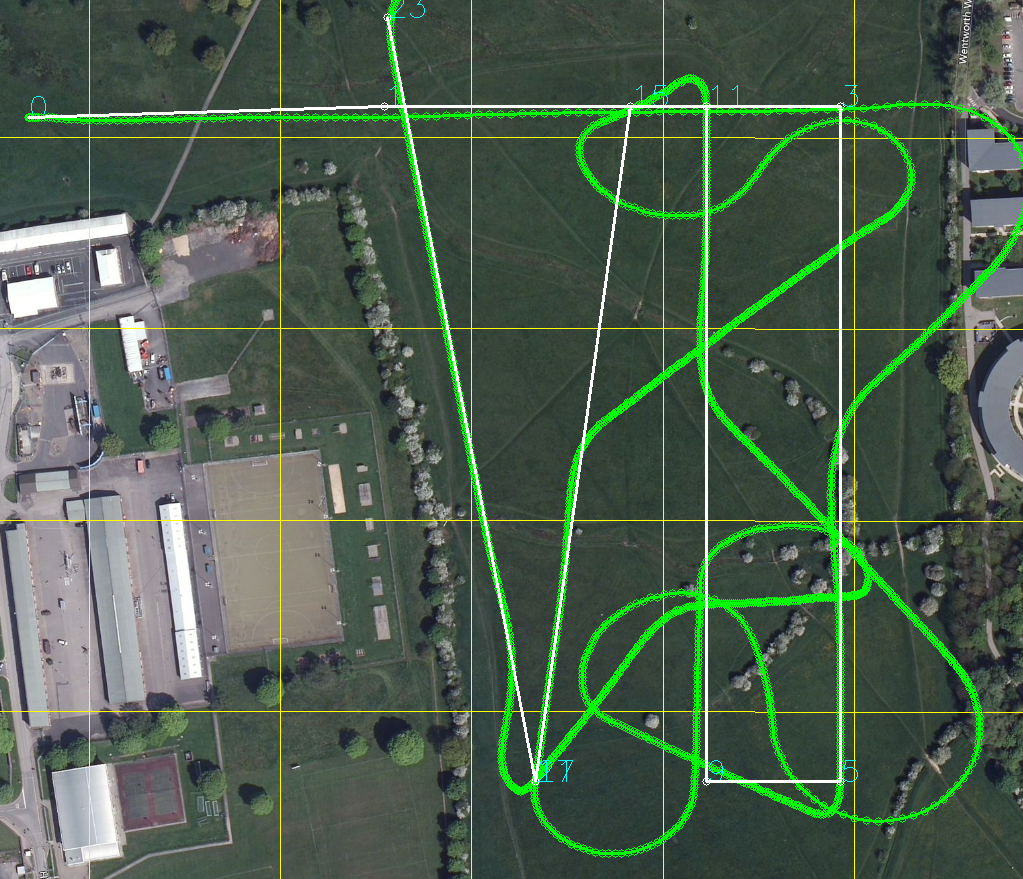
\includegraphics[width=\textwidth]{5Wind_32_20}
\caption[An attempt at flying Dubins path turns in wind]{The new system's failed attempt at flying Dubins path turns in wind to align with imaging paths}
\label{fig:3220withwind}
\end{figure} 

